\chapter{Problem Analysis}
\label{cha:problem_analysis}

This thesis focusses on a concrete example scenario. This helps to better understand the implications and advantages of the proposed method. Also the obtained results are more easily compared against the traditional approach.

A widely applicable scenario for modeling bones and soft tissue are fingers. The scenario being used in this thesis involves two fingers grabbing onto and lifting block of the ground. The fingers are positioned to the either side of the block in the model. While applying a continuous pressure onto the block the fingers are lifting it up from the floor and into the air. This is directly applicable to a number of different scenarios involving a robotic arm with attached fingers, which is supposed to pick up blocks are other objects of the ground.

\begin{figure}[htbp]
\centering
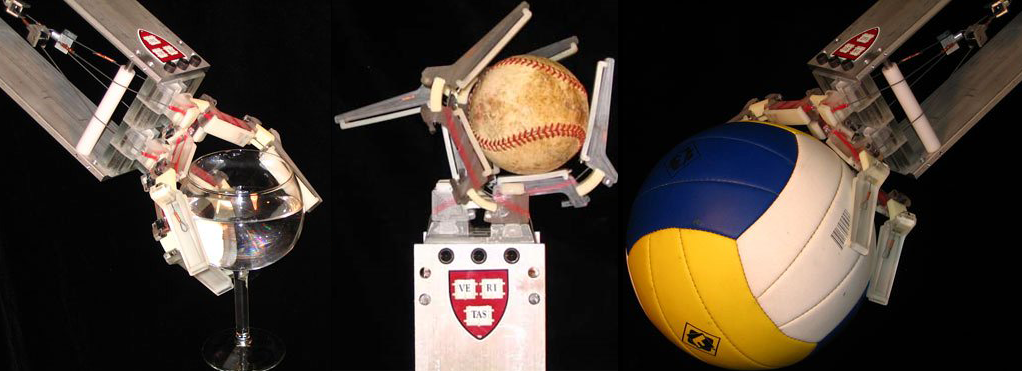
\includegraphics[width=.96\textwidth]{images/robot_grabbing.png}
\caption{Robotic hand picking objects up\protect\footnotemark}
\label{img:robot_grabbing}
\end{figure}
\footnotetext{http://www.yalescientific.org/2010/12/engineering-flexible-robotic-hands/}

All this has to be able to be simulated in realtime in order to be used games and animations. The simulations also has to be robust against numerically instabilities. These are either caused by simple numerical or rounding errors or by the fingers being slightly off the target when grabbing onto the block. Forces between the inner bone and outer tissue as well as forces between the tissue and other objects have to be modeled so a realistic result can be achieved. This is especially true for the friction caused by the tissue on the block, as otherwise the block would not be lift up at all.

Using a simple rigid body simulation for this is suboptimal. Both fingers and the block would be modeled as rigid bodies. Resolving all the resulting forces acting on the block can quickly get numerically unstable. The blocks can start to move and wiggle incorrectly until the results are no longer visually pleasing and physically plausible.

The problem is further complicated when instead of a simple block any kind of round object like a cylinder would have to be picked up. This would require the fingers to be touch the cylinder perfectly perpendicular and on the exact opposite points. Otherwise the pressure and the resulting forces would simply let the cylinder slip out either in front or the back. This is basically impossible to achieve numerically.

The way to traditionally solve this problem has been to use multiple rigid bodies to simulate the each finger to get a better grip on the object that is lifted up. This way complicates the simulations quite a bit as joints and and many more blocks have to be simulated. However the problem of slowing increasing numerically instabilities would still occur and might still be very hard to handle efficiently.

Solving the problem with only deformable bodies is theoretically possible, however this would not really capture the real world idea of a rigid bone structure with a surrounding soft layer of tissue. Simulating everything as a deformable body would not be very efficient. This would require a lot more computational resources, especially when considering to apply this to a complete skeleton. Great care has also be taken to ensure that some deformable parts are mostly behaving as rigid structures while still giving a physically plausible result.

Therefore the main requirements for the proposed technique of combining an inner core of rigid bodies with a soft layer of surrounding deformable material can be summarized as:

\begin{enumerate}
\item realtime simulation
\item	low number of bodies
\item only approximate orientation of the fingers relative to the block
\item collision handling/force propagation inside the body between "bone" and "tissue"
\item modeling friction between fingers and object
\end{enumerate}